\documentclass[../main.tex]{subfiles}
%!TEX root = ./analysisThrusterArms.tex
\graphicspath {{../}}

\begin{document}
\subsection{Thruster Arms} \label{thrustArms}

\begin{figure}[H]
	\centering
	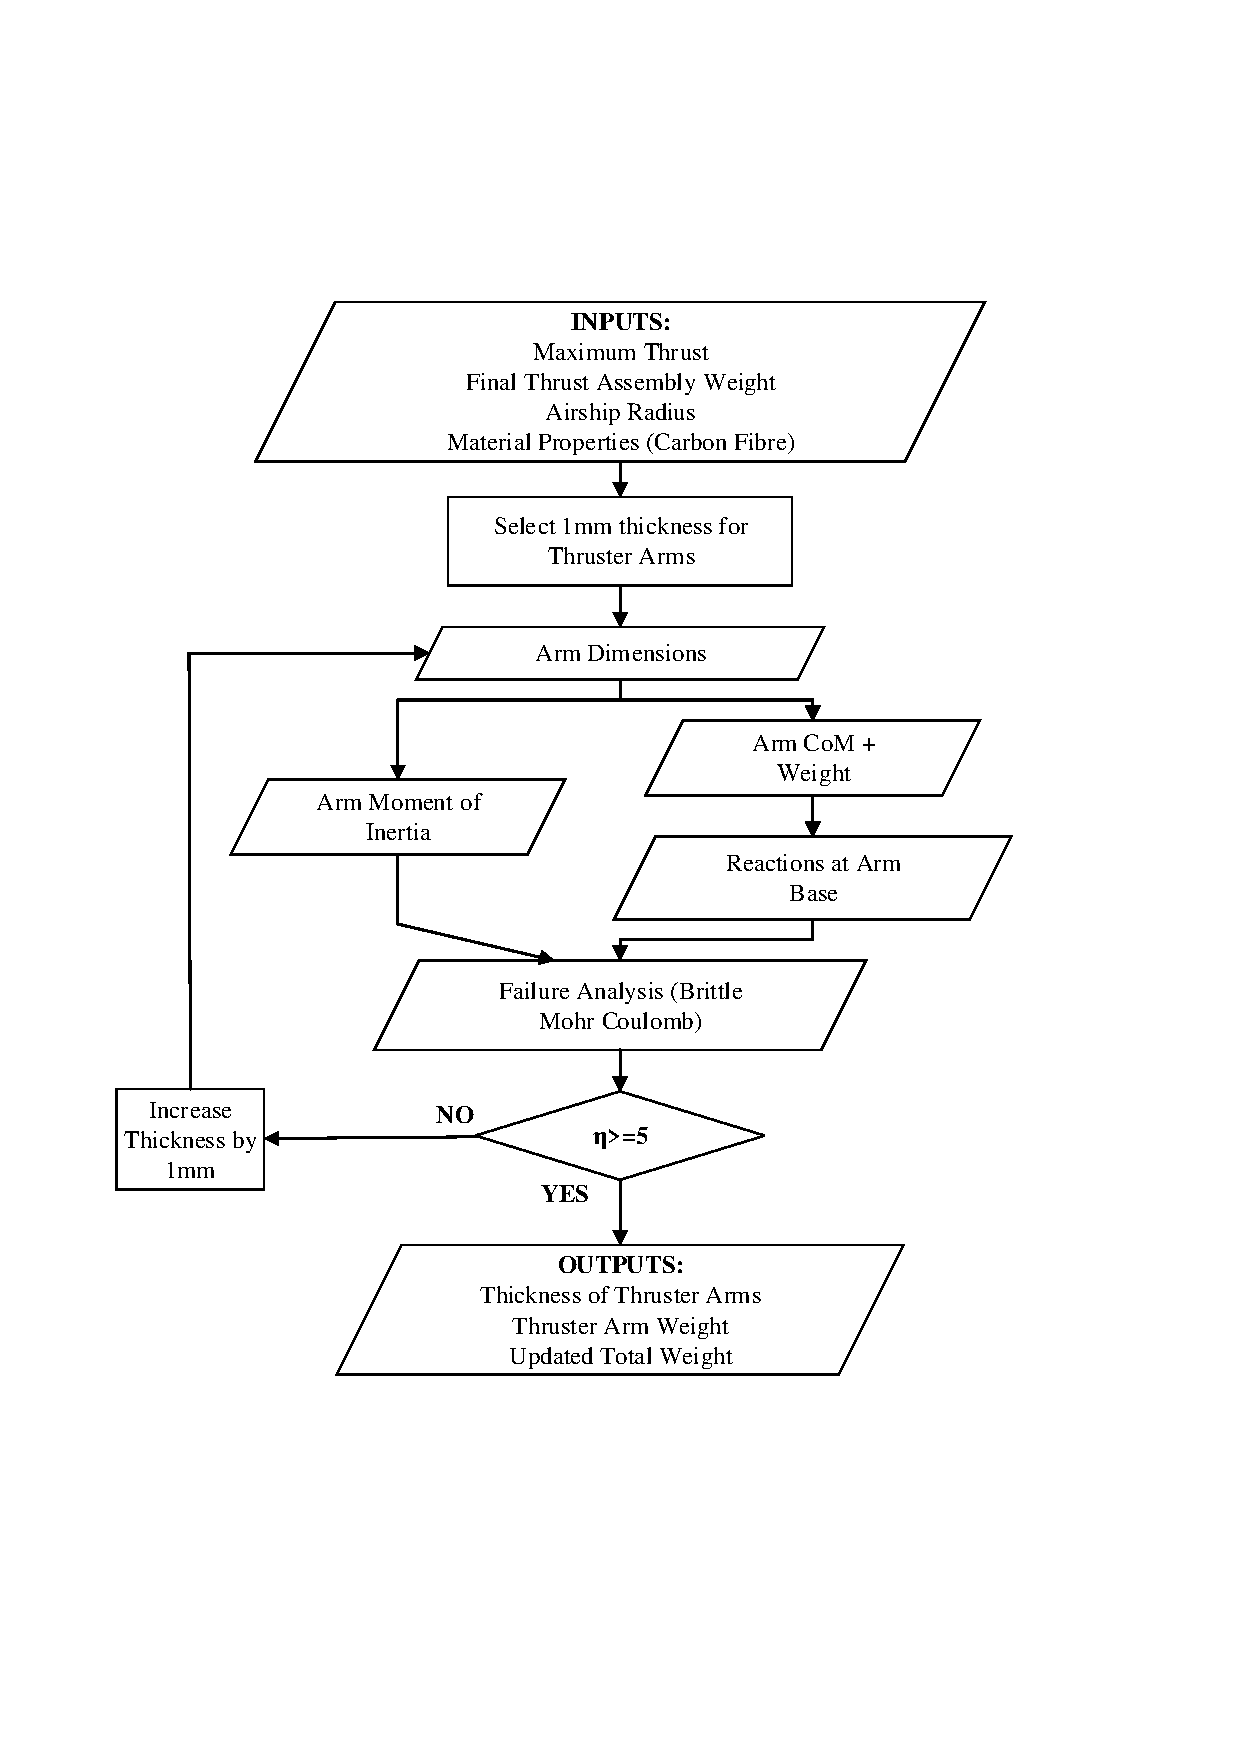
\includegraphics[width=.9\linewidth]{img/paramaterization/thrusterArms.pdf}
	\caption{Parametrization Outline for the Thruster Arms}
	\label{fig:thrusterArmsParametrization}
\end{figure}

The thruster arm analysis is performed to determine the required arm thickness to meet the specified safety factor. The analysis will calculate the weight and centre of mass then output the total mass of the arms and the thruster assembly it supports. In order to run the analysis several inputs are required including the maximum thrust force, thruster assembly weight, the airship radius, and the material properties of the carbon fibre the arms will be fabricated from. In order to minimize stress concentrations and increase ease of manufacturing the width of the arms is held constant and 30mm. This width enables the arms to remain the same width as the section where the keel connector is inserted as seen in FIG???. \\

The scenario for the analysis is that described in Loading Scenario, Section \ref{loadingScenarios} Maximum Downward Force shown in Figure \ref{fig:scenario1} where all forces are in $x$. The analysis begins by computing the reaction forces and moments at the point at the centre of the inner radius of the arms as seen in Figure \ref{fig:thrusterArmFBD}. These are calculated by solving the summation of forces from the Figure \ref{fig:thrusterArmFBD}.

\begin{figure}[H]
	\centering
	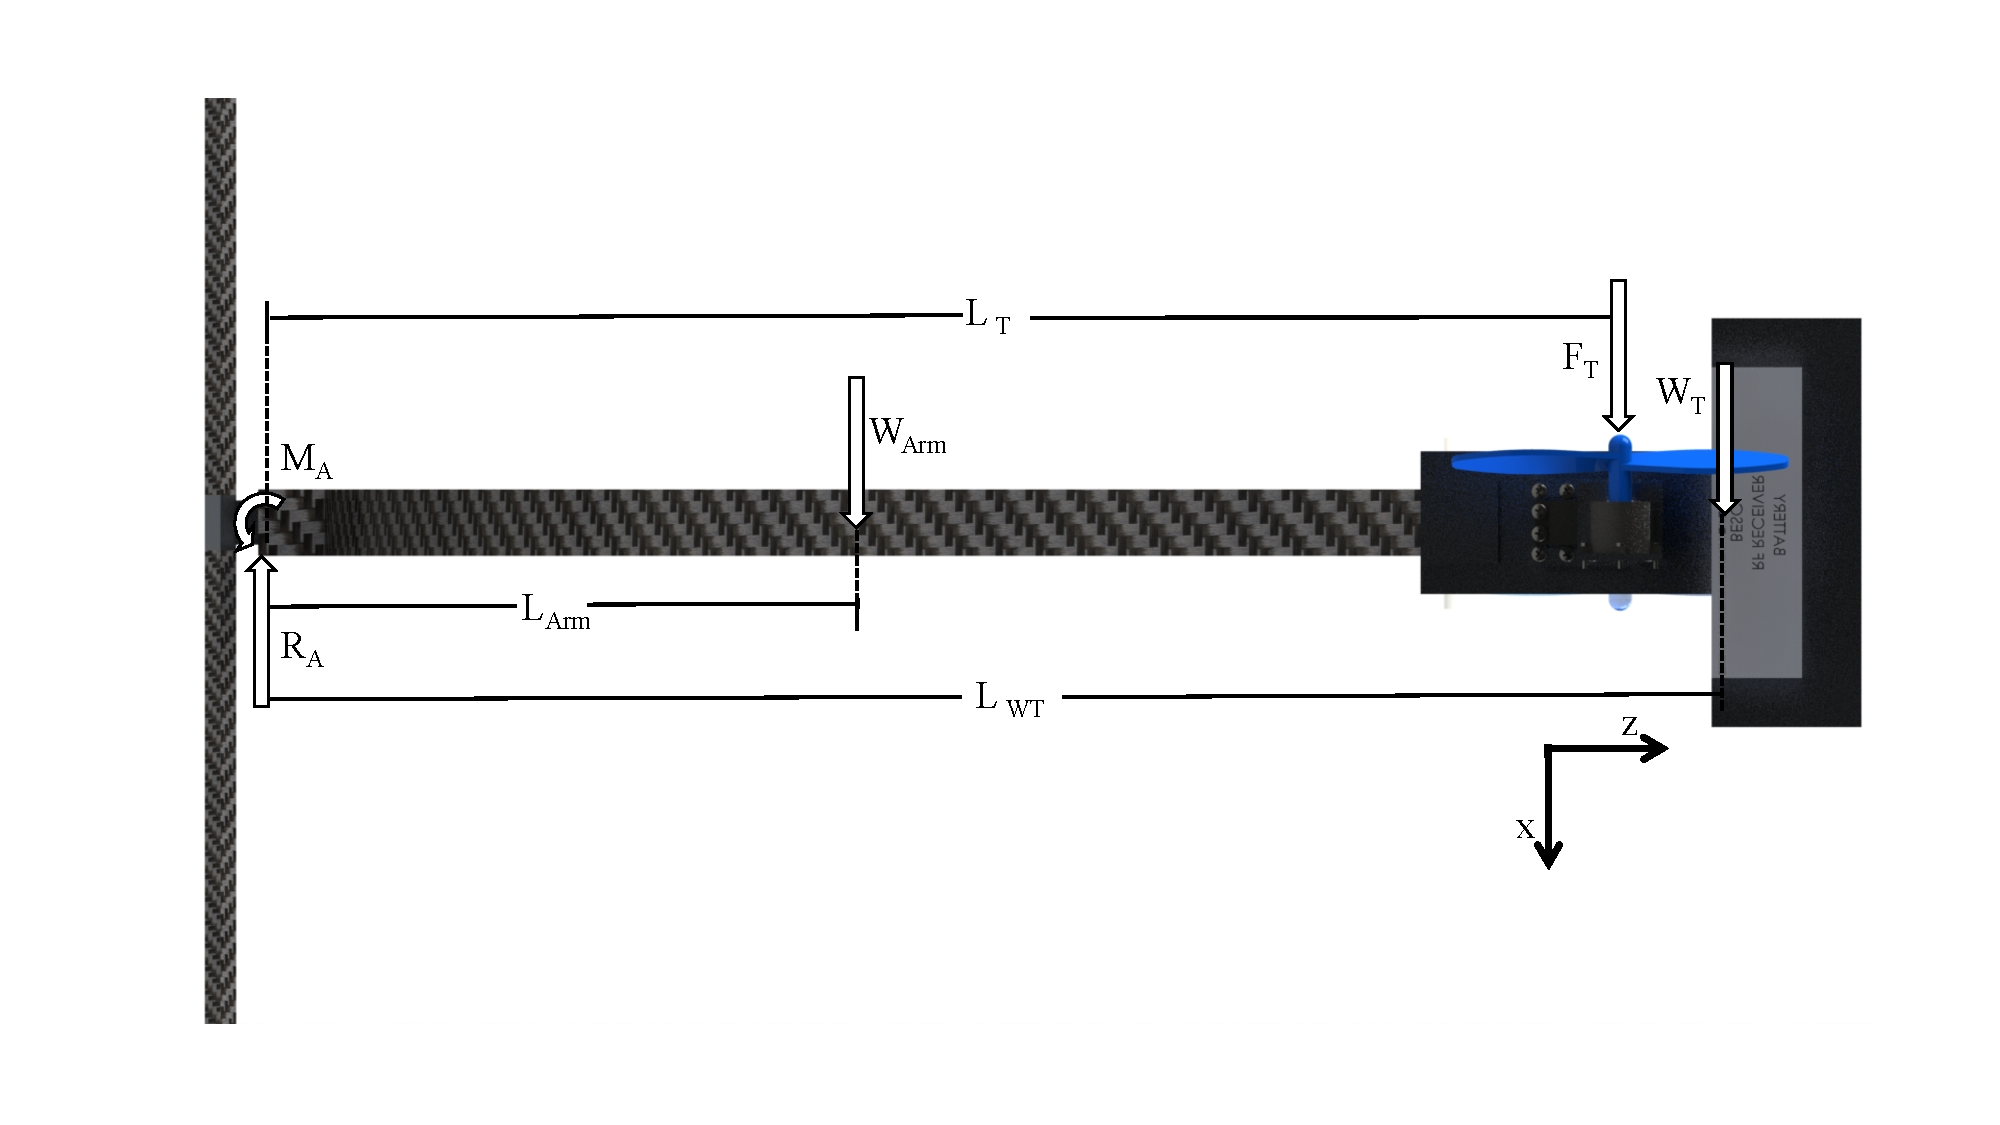
\includegraphics[width=.9\linewidth]{img/analysis/arm/thrusterArm.pdf}
	\caption{Free Body of the Thruster Shaft}
	\label{fig:thrusterArmFBD}
\end{figure}

The forces on Figure \ref{fig:thrusterArmFBD} are the thrust force ($F_T$), weight of thruster components ($W_T$), weight of the arm ($W_{Arm}$), and the reaction forces at the connector ($R_A$ and $M_A$). In the code the summation of forces is not used, using the forceSolver REF?? instead. However, for analysis done by hand, the summation of forces can be solved to get the reaction forces to find the stresses.

\begin{equation} \label{eqn:armFx}
\upplus \Sigma F_x = 0 = R_A - W_{Arm} - F_T - W_T
\end{equation}
\begin{equation} \label{eqn:armMA}
\curveplus \Sigma F_x = 0 = M_A - W_{Arm}(L_{Arm}) - F_T(L_T) - W_T(L_{WT})
\end{equation}

To get $W_{Arm}$ and $L_{Arm}$ the centre of mass of the arm has to be calculated each time the dimensions change. The following equation \ref{eqn:armCg} is used to solve for the centre based on the inner and outer radii $r_o$ and $r_i$. Because of symmetry, the centre of gravity in z is the same of that in y but negative. 

\begin{equation} \label{eqn:armCg}
W_{Arm} = \rho g\frac{0.03\pi(r_o^2 - r_i^2)}{4}, \quad L_{Arm} =\frac{4(r_o^3 - r_i^3)}{3\pi(r_o^2 - r_i^2)}
\end{equation}

Once the centre of mass is found the code uses forceSolver REF?? to find the reaction forces at the bottom of the arm. These reactions are used to calculate the stresses acting on the center of the inner radius surface shown in FIG ??. In initial design of the component all possible stresses were considered. These were used to find the worst case loading scenario and the location to take the stresses. The maximum stress occurs of the middle of the top of the cross section when the blimp is angled at $90°$. Subsequently this results in Equation \ref{eqn:armystress} being zero and having no effect on the safety factor. For analysis the planar stress in $y$ is calculated using the equation \ref{eqn:armystress} shown below. 
\begin{equation}
\label{eqn:armystress}
\sigma_{y}=  \underbrace{\frac{M_{x}c_z}{A r_i (\bar{r} - r)}}_\text{Bending moment stress about x} + \underbrace{\frac{M_{z}c_x}{I_z}}_\text{Bending moment stress about z} + \underbrace{\frac{F_y}{A}}_\text{Axial stress} 
\end{equation}
Where $A$ is the area, width $w$ times height $h$, $\bar{r}$ is the centre radius of the arm and $r$ is the neutral axis calculated by equations \ref{eqn:armNeutralAxis} shown below. $c_z$ is the distance to the neutral axis $r - r_i$. As mentioned above for this loading scenario $M_x = 0$, $c_x = 0$, and $F_y = 0$ resulting in the equation being 0.
\begin{equation} \label{eqn:armNeutralAxis}
\bar{r} = r_i + \frac{h}{2} \hspace{20mm}  r = \frac{h}{ln(r_o/r_i)}
\end{equation}
As mentioned above the primary stress acting on the arm is torsional shear. This is calculated using equation \ref{eqn:armtorsionShear} from {(Shigley's Machine Design \cite[102]{shigley})}. $M_y$ is the reaction moment at A, $w$ is the width of the arm, $h$ is the thickness of the arm.

\begin{equation} \label{eqn:armtorsionShear}
\tau_{XZ} = \dfrac{M_{y}}{wh^2}(3+\frac{1.8h}{w})
\end{equation}

Lastly, the analysis takes both the planar and shear stresses, then uses Cauchy's tensor to convert to principle stresses (Appendix \ref{appendix:cauchy}). These principle stresses are then used to determine the safety factor by Brittle Mohr-Coulomb Theory \cite[227]{shigley}. $\sigma_t$ is the ultimate tensile strength, $\sigma_c$ is the ultimate compressive strength, $\sigma_1$ is the first principle stress, and $\sigma_3$ is the third principle stress.

\begin{equation}
\eta = \frac{\sigma_t\sigma_c} {\sigma_c\sigma_1 -\sigma_t\sigma_3} \Rightarrow 5 \geq \frac{\sigma_t\sigma_c} {\sigma_c\sigma_1 -\sigma_t\sigma_3}
\end{equation}

A safety factor of five was chosen because there is a relatively high failure likelihood and due to their size they are prone to manufacturing defects.

\paragraph*{Sample Calculations}
$M_y$, $S_1$ and $S_3$ are taken from the MATLAB Force Solver program.
$$\tau_{XZ} = \dfrac{M_{y}}{wh^2}(3+\frac{1.8h}{w})= \dfrac{8.6098N\cdot{}m}{(0.030m)(0.0040m)^2}(3+\frac{1.8(0.0040m)}{(0.030m)})=58.12MPa$$

$$\eta = \dfrac{S_{ut}}{\sigma _a} = \dfrac{S_{ut}}{\sigma _a}$$

\end{document}